\documentclass{article}

% NeurIPS 2025 style files
\usepackage{neurips_2025}

% Standard packages
\usepackage[utf8]{inputenc} % allow utf-8 input
\usepackage[T1]{fontenc}    % use 8-bit T1 fonts
\usepackage{hyperref}       % hyperlinks
\usepackage{url}            % simple URL typesetting
\usepackage{booktabs}       % professional-quality tables
\usepackage{amsfonts}       % blackboard math symbols
\usepackage{amsmath}        % mathematical formulas
\usepackage{amssymb}        % mathematical symbols
\usepackage{nicefrac}       % compact symbols for 1/2, etc.
\usepackage{microtype}      % microtypography
\usepackage{xcolor}         % colors
\usepackage{graphicx}       % include graphics
\usepackage{subcaption}     % subfigures
\usepackage{algorithm}      % algorithms
\usepackage{algorithmic}    % algorithm formatting

% Title and authors
\title{
  Mechanistic Interpretability for Neural Interpretability: 
  A pipeline for interpretable, neural feature discovery
}

\author{%
  Author Name\thanks{Equal contribution} \\
  Department/Institution \\
  Address \\
  \texttt{email@institution.edu} \\
  % Add more authors as needed
  % \And
  % Co-Author Name\footnotemark[1] \\
  % Department/Institution \\
  % Address \\
  % \texttt{email@institution.edu} \\
}

\begin{document}

\maketitle

\begin{abstract}
Understanding neural computations requires identifying interpretable features from large-scale neural recordings. We present a novel application of Multi-Scale Sparse Autoencoders (MSAEs) to neural data analysis, enabling the discovery of interpretable latent features across multiple temporal and spatial scales. Our approach combines traditional Sparse Autoencoders (SAEs) with multi-scale architectures to extract meaningful neural representations from high-dimensional neural recordings. We evaluate our method on multiple large-scale datasets including Allen Neuropixels visual coding data, Churchland datasets, and Aeon recordings. Our results demonstrate that MSAEs can identify biologically relevant features while maintaining reconstruction quality, offering new insights into neural computation patterns. The discovered features show improved interpretability compared to traditional dimensionality reduction methods and enable effective decoding of behavioral and stimulus variables.
\end{abstract}

% Include individual sections
\section{Introduction}

Advanced extracellular recording technologies now enable neuroscientists to capture unprecedented volumes of high-dimensional neural\footnote{By default, "neural" and "neuron" will refer to neurobiology; e.g. we may call biological neuronal spike data "neural activity". In contrast, activity and neurons from artificial neural networks will be explicitly prefaced; e.g. "artificial neural activity" or "the model's neurons".} data at single-cell resolution ~\cite{steinmetz_2021_neuropixels2, raducanu_2017_neuroseeker, cai_2016_miniscope, villette_2019_voltage_2p, ouzounov_2017_three_photon, ahrens_2013_lightsheet}. Understanding the computational principles driving neural activity requires extracting interpretable features from this data. Traditional dimensionality reduction techniques, while useful for visualization and basic analyses, often make invalid assumptions about or altogether fail to disentangle distributed representations, and as a result typically cannot provide a mechanistic understanding of the underlying computations ~\cite{cunningham_2014_neural_dr, humphries_2021_dr_principles}. Recent work has produced promising latent variable model (LVM) approaches capable of identifying low-dimensional subspaces that can accurately decode aspects of behavior and environment ~\cite{song_2025_langevinflow, schneider_2023_cebra, le_2022_stndt, keshtkaran_2022_autolfads, yu_2009_gpfa, macke_2011_plds, gao_2016_pflds, low_2018_mind, jensen_2020_mgplvm, hernandez_2020_vind, kim_2021_plnde, hurwitz_2021_tndm, schimel_2022_ilqrvae, kudryashova_2023_ctrltndm, ye_2023_ndt2, gondur_2024_mmgpvae, pellegrino_2024_slicetca, sani_2024_dpad, pals_2024_smclr_rnn, zhang_2024_mtm, george_2025_simpl, perkins_2025_mint, schmutz_2025_nce}. However, these methods typically value decoding accuracy over latent interpretability, and consequently all have at least one of the following limitations: poorly interpretable latents, lossy mapping to and/or poor reconstruction of neural data from latent space, priors on the latent and/or neural data space, requirements of additional behavioral, environmental, and/or trial-structured neural data, supralinear scaling with respect to dataset size, or high implementational complexity.

We address each of these limitations in MINI, which provides a simple, user-friendly library for interpretable latent discovery from high-dimensional neural data. We consider a latent's interpretability in two key aspects: 1) its correspondence to a specific external variable -- a "natural" behavioral or environmental feature\footnote{A "feature" is a sufficiently interpretable latent. We illustrate this in \nameref{section:results}.}; 2) its explicit composition from contributing neural activity. MINI's approach obviates the need for post-hoc analyses to find meaningful dynamics in latent spaces typical of other approaches. Additionally, while we showcase MINI on spike data, it can be readily used with virtually any other neural recording modality as the only data requirement is any predefined spatiotemporal binning.

At MINI's core is the training of shallow sparse dictionary neural network (SDNN) models whose individual dictionary elements -- hidden layer neurons -- ideally serve as interpretable latents. This particular LVM approach has had many successes in the field of AI mechanistic interpretability ~\cite{cunningham_2023_saes, bricken_2023_towards_monosemanticity, templeton_2024_scaling_monosemanticity, ameisen_2025_circuit_tracing, lindsey_2025_biology_llm}, and here is additionally motivated by the principle that we need not explicitly impose structure on the latent space nor model its dynamics to discover interpretable variables. Specifically, MINI bypasses the need to enforce non-Markovian dynamics, which are often a property of an incomplete observation of a system rather than the system itself; any dynamical system can be represented as Markovian via sufficient state augmentation ~\cite{takens_1981_embedding}. Given this, even methods that appear non-Markovian can be seen as attempts to approximate a complete underlying state. For example, the forward dynamics of a recurrent neural network (RNN) are Markovian in its hidden state ~\cite{sussillo_2013_rnn_dynamics, goodfellow_2016_rnn}, and generalized linear models (GLMs) with history filters ~\cite{pillow_2008_glms, truccolo_2005_pointprocess} use past activity to augment the present state. This perspective aligns with several findings in neuroscience, from activity in motor cortex reflecting a low-dimensional, implicitly Markovian dynamical system ~\cite{churchland_2012_population_dynamics, shenoy_2013_dynamical_perspective}, to predictive-coding formulations that posit that the brain maintains an internal state sufficient to predict sensory streams, i.e., a Markovian latent process \cite{rao_1999_predictive_coding, doya_2007_bayesian_brain, friston_2010_free_energy}. Grounded in this perspective, MINI forgoes the challenge of modeling intricate dynamics and instead directly extracts meaningful constituent features of the underlying neural state (\autoref{figure:interpretable_latents_vs_latent_space}).

\begin{figure}[h]
    \centering
    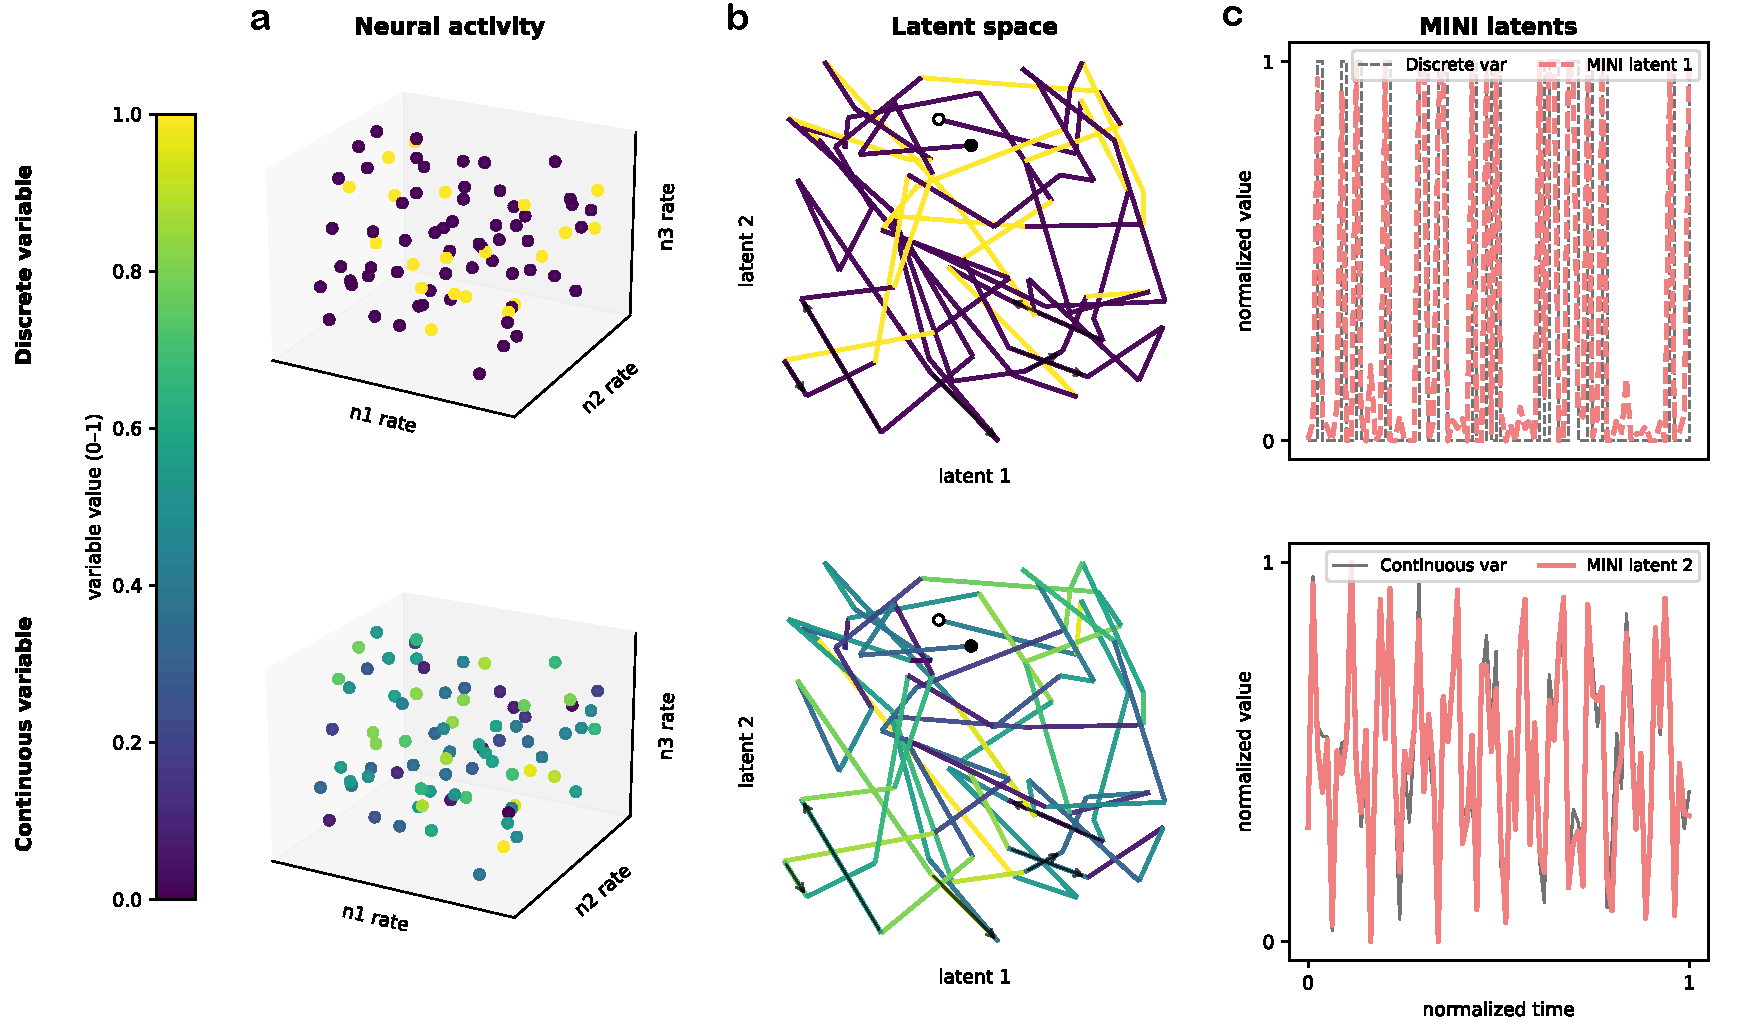
\includegraphics[width=\linewidth]{figures/interpretable_latents_vs_latent_space.pdf}
    \caption{
        \textbf{Interpretable latents vs. latent space.} \\
        \small This toy example highlights the utility of MINI. The two rows show two different variables (top: discrete; bottom: continuous), each uniquely encoded by the same underlying neural activity made up of three neurons' firing rates. The viridis colorbar shows the variables' values as a function of this neural activity. (\textbf{a}) Each point in the scatterplots represents a moment in time. (\textbf{b}) A projection of this activity into a 2D latent space creates tangled trajectories where variable states (e.g. 'on' and 'off' in the discrete case, and 'high' and 'low' in the continuous case) are not easily distnguished. The start and end points of the trajectories are marked by white and black dots, respectively, while arrows indicate trajectory direction. (\textbf{c}) In contrast to the tangled latent space, MINI finds individual latents corresponding to each variable, demonstrating the potential for improved interpretability of neural representations.
    }
    \label{figure:interpretable_latents_vs_latent_space}
\end{figure}
\section{Methods: The MINI pipeline}

\begin{figure}[h]
    \centering
    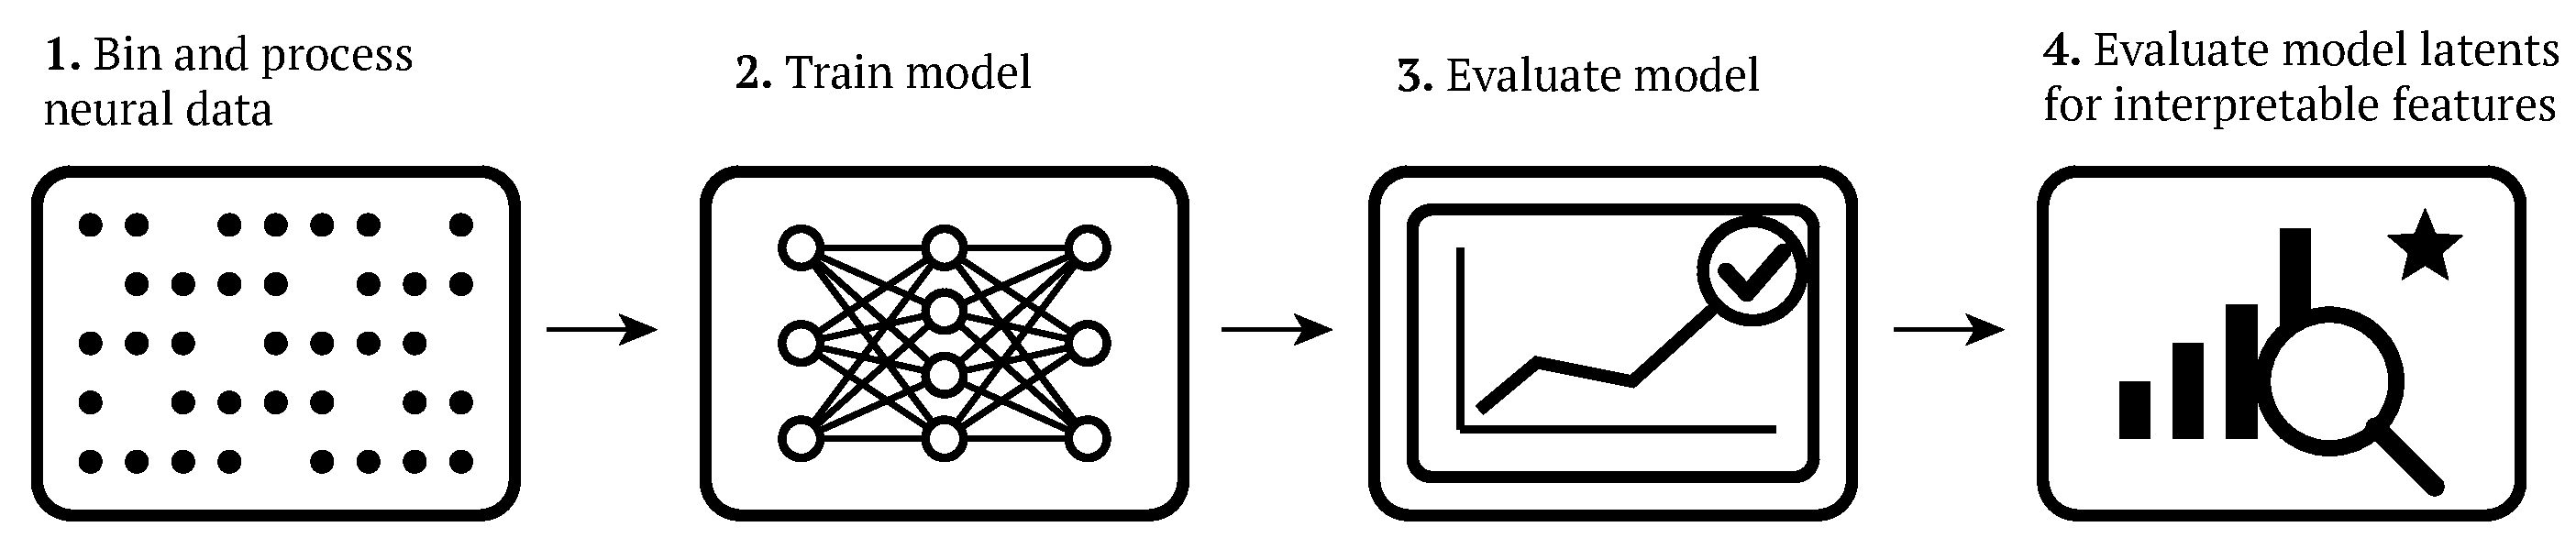
\includegraphics[width=\linewidth]{figures/mini_pipeline.pdf}
    \caption{
        \textbf{The MINI pipeline.} \\
        \small The MINI pipeline is comprised of 4 stages: 1) Spatiotemporal binning and processing of neural data; 2) Model training; 3) Model evaluation; 4) Latent evaluation for feature interpretability. Steps 1-3 can be either semi- or fully-automated.
    }
    \label{figure:mini_pipeline}
\end{figure}

The MINI pipeline transforms high-dimensional neural data into a set of interpretable latents in four primary stages (\autoref{figure:mini_pipeline}), the first three of which can be fully automated.

\subsection{Data preprocessing}

The pipeline's first stage prepares neural data for model training. MINI includes utilities to process outputs from common spikesorters (e.g. Kilosort ~\cite{pachitariu_2016_kilosort}) by aggregating, binning, and normalizing spike times into a 2D matrix of time by space, in which each bin contains neural activity from a neural unit for a specific time period. Normalization operations include min-max and z-scoring, applied across either the spatial or temporal dimension. This processing is readily adaptable to other forms of acquired neural data, such as ROIs from calcium imaging data processed by tools like Suite2p ~\cite{pachitariu_2017_suite2p}. Alternatively, users may pass their own preprocessed neural data directly to the model training stage.

\subsection{Model training}

In stage 2, a SDNN model is trained to reconstruct the processed neural data from latent, sparsely active dictionary elements -- the model's hidden layer neurons\footnote{In a SDNN model: model neuron = dictionary element = latent}. The end goal is for these latents to represent disentangled, interpretable representations\footnote{In our vernacular: interpretable latent $\approx$ feature $\approx$ representation} encoded by the neural activity (\autoref{figure:sdnn_arch}a,b). Sparsity encourages the model to discover a monosemantic dictionary, in which each latent corresponds to a single feature. For instance, a latent from a model trained on visual cortex activity may correspond to a particular property of a visual stimulus, while a latent from a model trained on motor cortex activity may correspond to a specific aspect of movement.

The model can be configured in three ways ~\cite{lindsey_2024_crosscoders}, depending on the relationship between the input and target neural data:
\begin{itemize}[nosep, leftmargin=1em, topsep=-0.5em]
    \item \textbf{Autoencoder}: The model reconstructs its own input; e.g. V1 activity based on V1 activity.
    \item \textbf{Transcoder}: The model reconstructs a dependent target of its input; e.g. V2 activity based on V1 activity.
    \item \textbf{Crosscoder}: The model reconstructs a related target of its input; e.g. V1 activity on day 2 based on V1 activity on day 1.
\end{itemize}
In all cases, the model is trained to minimize the difference between the reconstructed and actual target neural data. The full training procedure is summarized in \nameref{algorithm:sdnn_model_training}. Three key components are particularly worth noting: the batch top-$k$ sparsity, Matryoshka architecture, and optional integration over latent space history via self-attention.

A batch top-$k$ operator preserves only the $k \cdot B$ latents with the highest activation magnitudes across a batch of size $B$. This approach directly controls sparsity without a tunable regularization coefficient (e.g., an L1 penalty) and flexibly permits the number of active features to vary per sample in the batch, aligning with the variable complexity of neural states. A novel variant of the Matryoshka SDNN architecture ~\cite{bussmann_2025_msae} segments the latent space into hierarchical levels, where each level attempts a full reconstruction of the target neural activity (\autoref{figure:sdnn_arch}c). This allows for multi-scale feature representation at single timepoints, and mitigates "feature absorption," a common issue where general features subsume specific ones ~\cite{chanin_2024_feature_absorption}. For example, our model can learn that a "drifting grating" is a subset of the more general "grating" visual stimulus class without sacrificing the representation of either (\nameref{subsubsection:allen_dataset_results}). Lastly, if input data is provided as a sequence of timebins rather than single timebins, an optional transformer block can integrate information over the latent space history via self-attention, enabling the model to learn features corresponding to evolving temporal dynamics, rather than just instantaneous neural patterns. We find that in some cases the combination of these three components empirically improves both reconstruction accuracy and feature interpretability (see \nameref{subsubsection:architecture_details}).

Model training can be fully automated via a hyperparameter sweep configuration to train an optimal model over one or multiple local or distributed cpus or gpus. We typically sweep over key parameters such as the number and size of Matryoshka levels (n\_levels, dsae\_levels), the sparsity coefficient (topk), and the latent space sequence length. Depending on the optimizer used, it's recommended to additionally sweep over hyperparameters such as learning rate (we use Adam by default bc...)

\begin{figure}[htbp]
    \begin{minipage}{0.63\linewidth}
    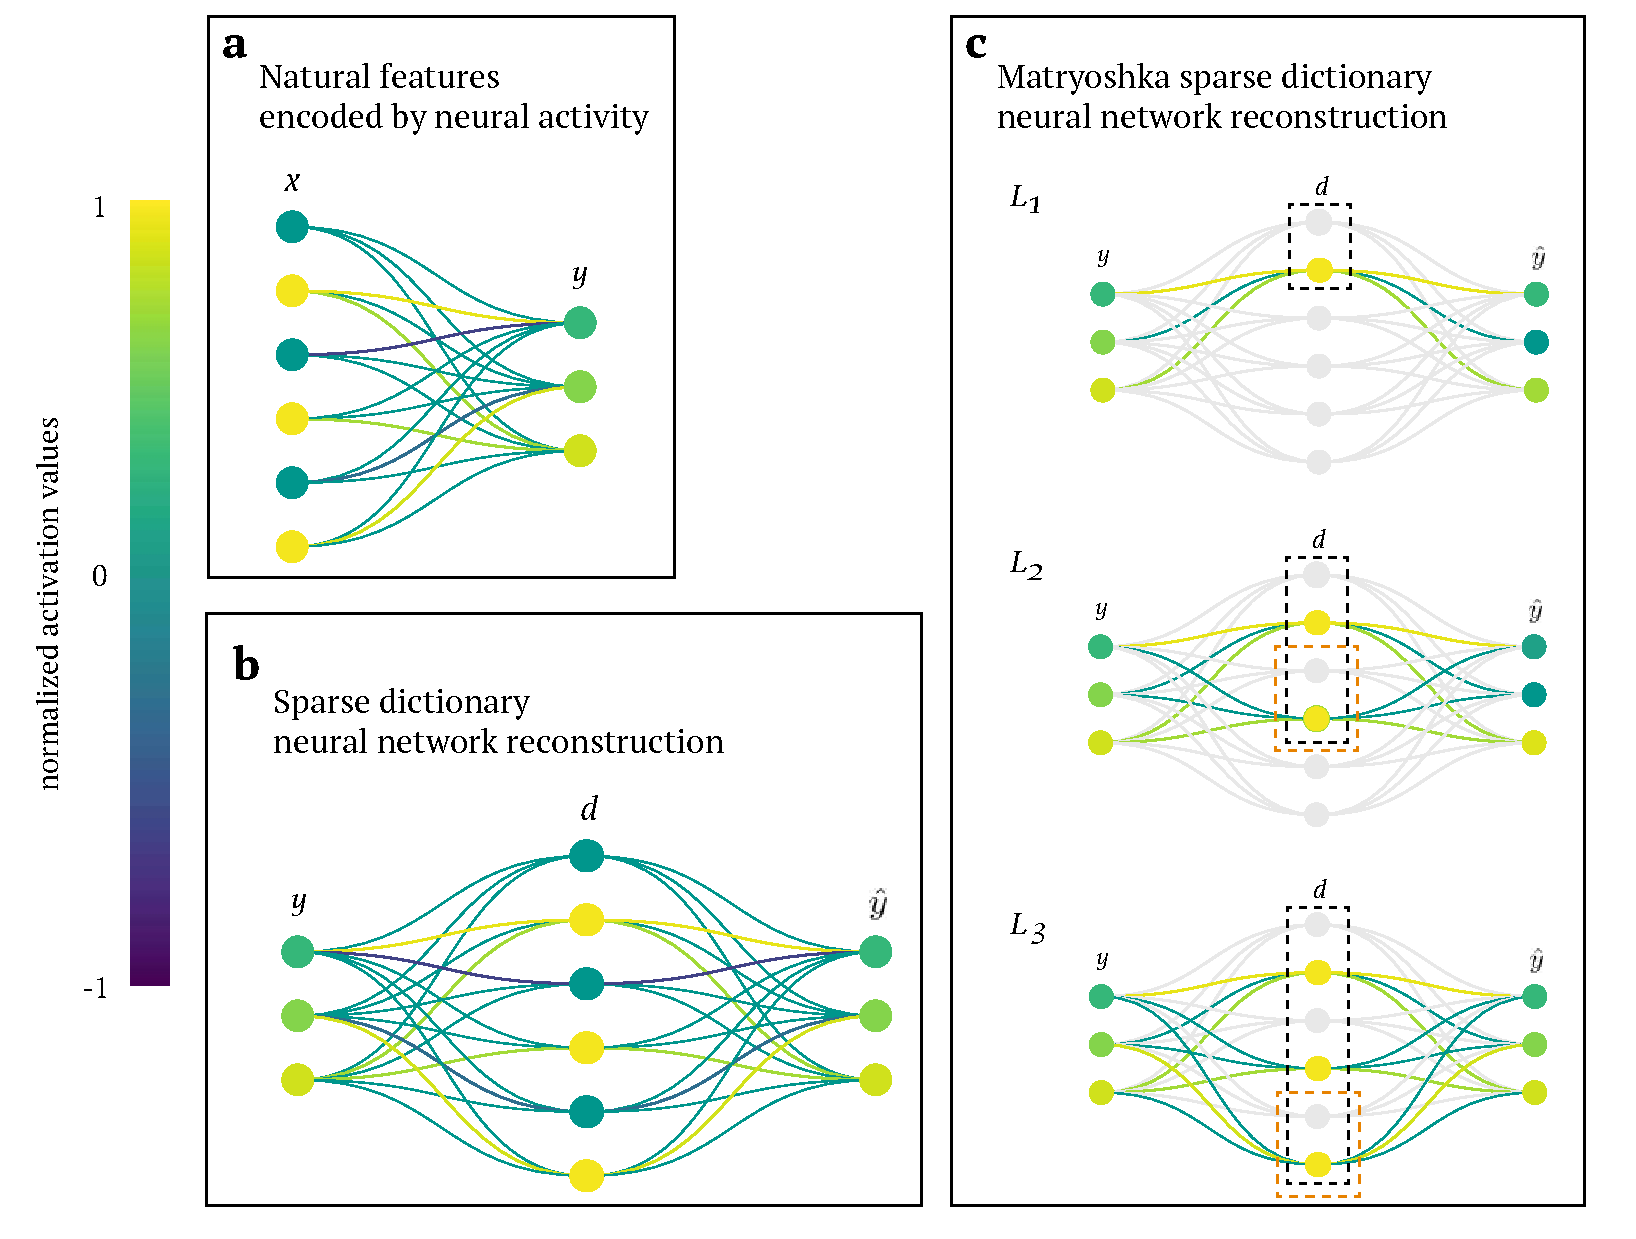
\includegraphics[width=\linewidth]{figures/sdnn_arch.pdf}
    \end{minipage}%
    \begin{minipage}{0.37\linewidth}
    \caption{
        \textbf{Model motivation} \\
        \small
        (\textbf{a}) Natural, "real-world" features $x$ are encoded by neural activity $y$. In this example, three active features are simultaneously represented by the joint activity of three neurons. (\textbf{b}) A SDNN reconstructs neural activity $z$ based on $y$ via sparse dictionary elements $d$. When training is successful, $d$ corresponds to $x$: sparse dictionary elements (i.e. model neurons) represent natural features. If $z$ tries to recreate $y$ exactly ($\hat{y}$), the model is an autoencoder; in other scenarios (e.g. $z$ is separate but dependent on or related to $y$) it is a transcoder or crosscoder. (\textbf{c}) A Matryoshka SDNN segments the latent space into multiple levels, each of which attempts to do a full reconstruction of the target neural activity. The black boxes indicate the latents involved in a single level, while the light-red boxes indicate the additional latents used at lower-levels. A $k = 1$ value is chosen for top-$k$ selection of the total possible additional latents to recruit for reconstruction at each level (the yellow neuron within each light-red box). Latents in the highest-level ($L_1$) will often correspond to high-level features (e.g. a round object), while latents exclusive to the lowest-level ($L_3$) will often correspond to low-level features (e.g. a basketball).
    }
    \label{figure:sdnn_arch}
    \end{minipage}
\end{figure}

\hrule
...
\hrule

In step 3, the trained model is evaluated using a variety of metrics to assess its performance. (SAEBench ~\cite{karvonen_2025_saebench}) If the model does not meet the desired criteria, it can be re-trained with different hyperparameters.

\begin{figure}[h]
    \centering
    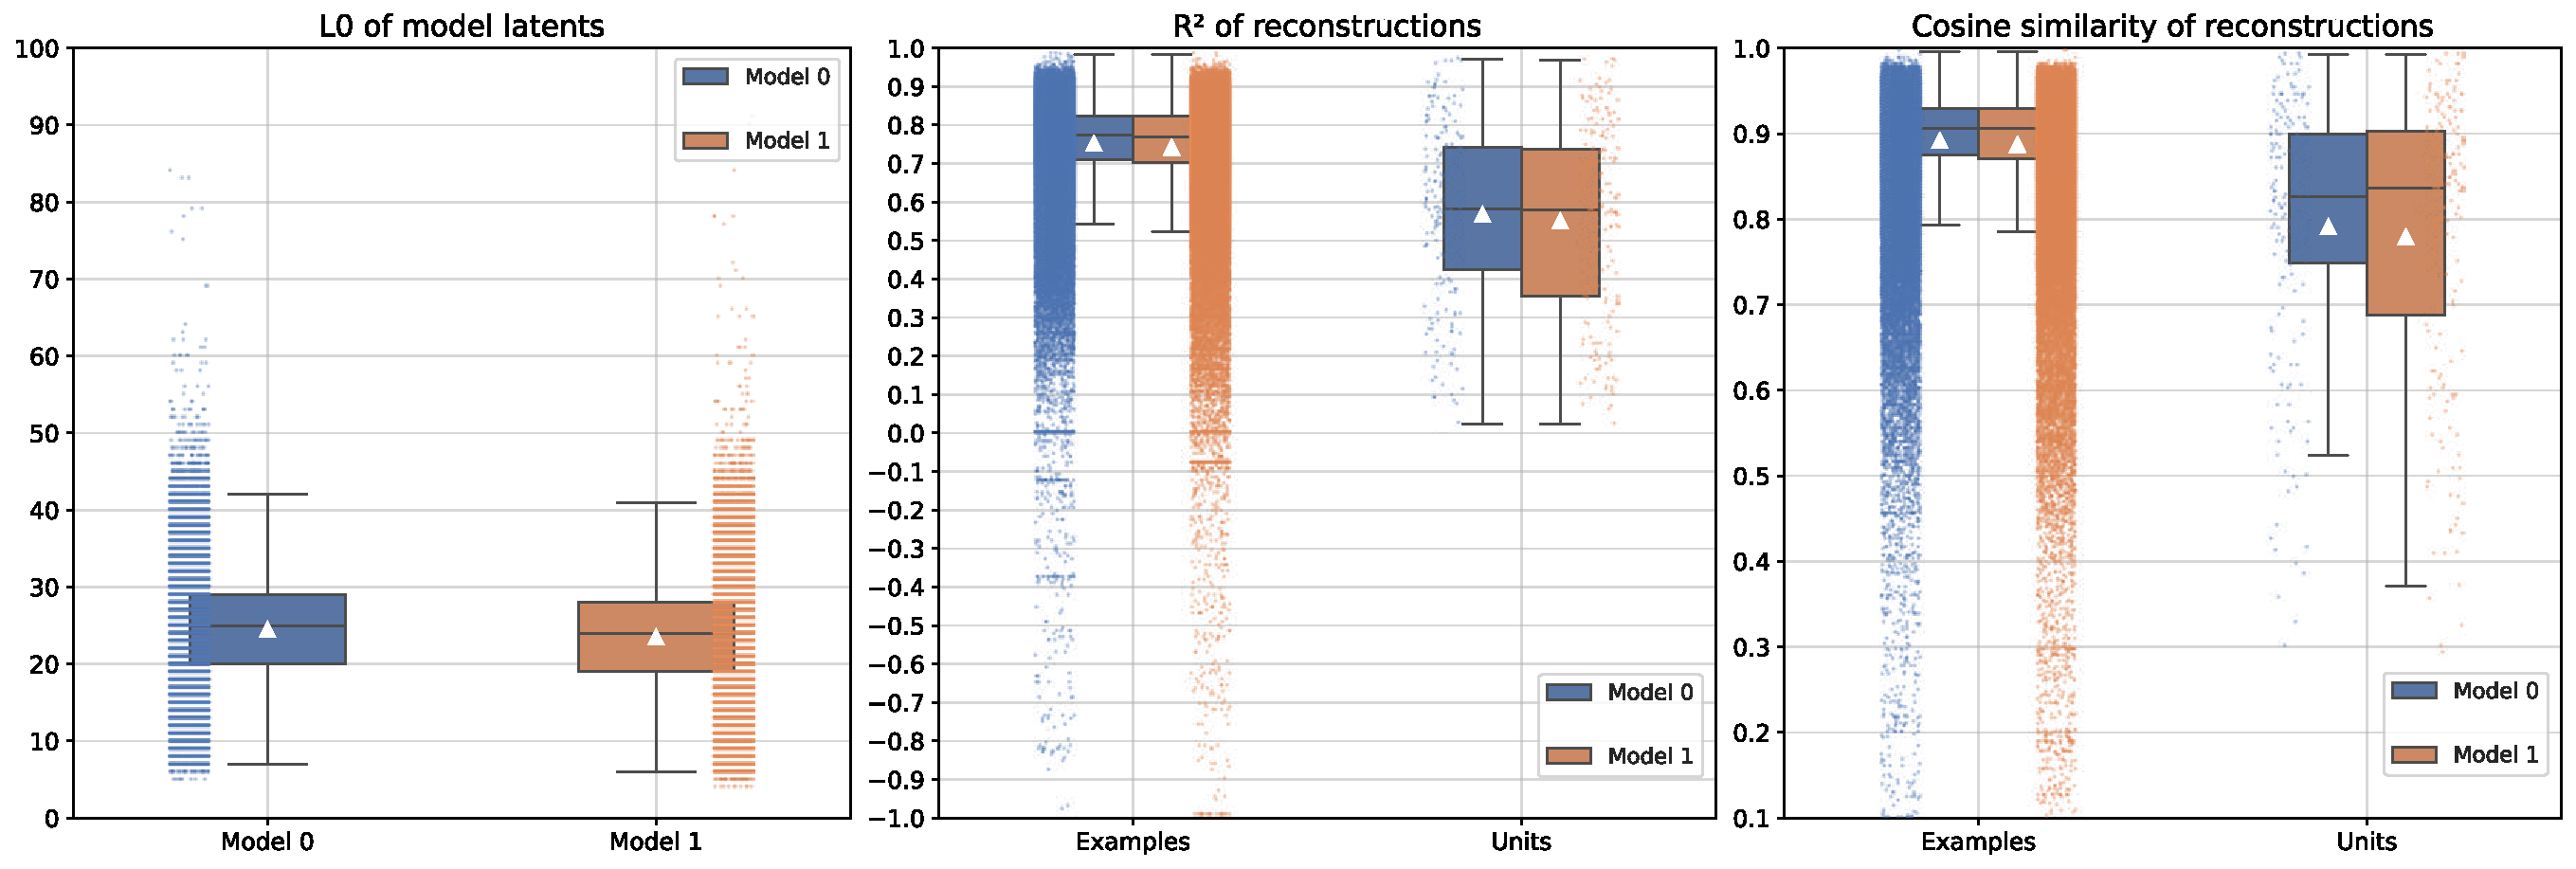
\includegraphics[width=\linewidth]{figures/model_eval.pdf}
    \caption{
        \textbf{Model evaluation metrics.} \\
        \small By default, trained models are evaluated via the following metrics: latent L0 (left), and R\textsuperscript{2} (middle) and cosine similarity (right) of reconstruction-to-actual neural activity for each temporal ("Examples") and spatial ("Units") bin. ... Additional features, such as the R\textsuperscript{2}of overall neural data reconstruction for each individual latent, can be specifed and included.
    }
    \label{figure:model_eval}
\end{figure}

Finally, in step 4, the latents produced by the model are evaluated for interpretability as features. This includes visualizing their activation patterns over time and experimental conditions, as well as assessing their decoding performance. We detail typical approaches to feature evaluation in \nameref{section:results}.

\hrule
...
\hrule

- For a user, the full, semi-automated pipeline is as follows:
\begin{enumerate}
    \item Data processing
    \begin{itemize}
        \item Spatiotemporally bin and normalize
        \begin{itemize}
            \item MINI has a convenience function to do this directly from output of common spikesorters (kilosort), where we bin unit spikes given a specified timebin and optionally normalize (z-score or max) dataset across time and/or unit
            \begin{itemize}
                \item (and similar approach could be applied to output from common calcium imaging processing (e.g. Suite2p))
            \end{itemize}
        \end{itemize}
    \end{itemize}
    
    \item Model training
    \begin{itemize}
        \item Hyperparameter optimization
        \begin{itemize}
            \item Model parameters
            \item Optimizer parameters
        \end{itemize}
        \item By default no validation set, but can be added if we want to e.g. apply to other recordings of same animal, though this is not generally recommended (just train a freshie)
    \end{itemize}
    
    \item Model evaluation
    \begin{itemize}
        \item (We implement all metrics from SAEBench which are not language-model specific, plus a couple of our own)
        \item L0 of latents
        \item R\textsuperscript{2} (var explained) and cos sim of reconstruction-to-actual neural activity for each spatial bin, and each temporal bin
        \item Latent density histogram (as in SAEBench)
        \item Variance explained of overall reconstruction from each latent (variance shouldn't be in just a few features) ?
        \item Spectral frequency analysis to ensure temporal frequency content is preserved?
    \end{itemize}
    
    \item Feature evaluation
    \begin{itemize}
        \item When a latent is subjectively determined to be sufficiently interpretable, we call this a feature.
        \item Interactive plots showing feature activation patterns across time and experimental conditions.
        \item We evaluate its decoding performance?
        \item Export functionality.
    \end{itemize}
\end{enumerate}

\section{Results}
\label{section:results}

- We evaluate MINI on one synthetic single-unit dataset with ground-truth latents, and three real extracellular electrophysiology, open-source, high-yield, single-unit datasets, across multiple, distinct brain regions in multiple species. (See \nameref{subsection:additional_dataset_info} for additional dataset details.)

- Overall, we show that MINI can:
\begin{enumerate}
    \item Discover discrete and continuous, environmental and behavioral features
    \item Robustly find same features across time and subjects.
    \item Find features across different timescales (i.e. that persevere for different durations)
    \item Find hierarchical features.
\end{enumerate}    

- On the synthetic dataset, we show that MINI can recover all ground-truth latents, and use them to decode natural features of interest.

- On one natural dataset, we compare MINI to other popular approaches that have also been applied to the same dataset, and show that MINI more clearly reveals certain features than these other methods, while maintaining high reconstruction and decoding accuracy.

- On the other two natural datasets, we show that MINI can reveal expected and unexpected features (optinally / time-permitting, that CEBRA and LangevinFlow don't find), highlighting its use as a powerful tool for neuroscientific discovery.

---

\subsection{Simulated rat spike data in a navigation task}

...

\subsection{Churchland Motor Cortical Datasets}

\subsubsection{Dataset Overview}

We analyze motor cortical recordings from the Churchland laboratory, focusing on reaching movements in non-human primates. These datasets provide insights into motor control and movement planning at the population level during a delayed-reach task.

\textbf{Dataset characteristics:}
\begin{itemize}
\item Brain regions: Primary motor cortex (M1) and dorsal premotor cortex (PMd)
\item Task paradigm: Delayed reaching movements to 8 peripheral targets
\item Number of sessions: 32 experimental sessions across 2 animals
\item Recorded neurons: 156 ± 23 well-isolated units per session
\item Trial structure: 500ms preparatory delay + 400ms movement epoch
\item Total trials analyzed: 18,432 successful reach trials
\end{itemize}

\subsubsection{Motor Control Feature Discovery}

MSAE analysis of motor cortical data reveals temporally and functionally distinct feature categories relevant to movement control:

\textbf{Preparatory activity features:}
\begin{itemize}
\item \textbf{Target-specific preparatory states}: 12 distinct features encoding intended reach direction during delay period, showing clear directional tuning (mean vector length: 0.73 ± 0.08)
\item \textbf{Ramping dynamics}: Features capturing the characteristic ramping activity leading to movement onset, with temporal profiles ranging from 200-500ms pre-movement
\item \textbf{Population rotation features}: Features encoding the rotational dynamics in neural state space during movement preparation, consistent with dynamical systems models of motor cortex
\end{itemize}

\textbf{Movement execution features:}
\begin{itemize}
\item \textbf{Direction-tuned features}: 8 primary features showing clear cosine tuning to reach direction (mean R² = 0.81 ± 0.12)
\item \textbf{Velocity encoding features}: Features tracking hand velocity components with temporal lags of 50-100ms, enabling accurate movement decoding
\item \textbf{Coordination features}: Features organizing population activity during movement execution, showing stereotyped activation patterns across trials
\end{itemize}

\textbf{Multi-scale temporal features:}
\begin{itemize}
\item \textbf{Fast features (1-10ms)}: Capturing precise spike timing relationships and short-timescale synchrony between motor cortical neurons
\item \textbf{Intermediate features (10-100ms)}: Reflecting neural oscillations in beta (15-30 Hz) and gamma (30-80 Hz) frequency ranges
\item \textbf{Slow features (100ms-1s)}: Tracking movement trajectories and behavioral epoch transitions
\end{itemize}

\subsubsection{Comparison with Established Methods}

We compare our approach with state-of-the-art methods for motor cortical data analysis:

\textbf{vs. Factor Analysis (FA):}
\begin{itemize}
\item MSAE features show 2.8× clearer separation between preparatory and movement periods
\item Better preservation of single-trial dynamics (trial-to-trial correlation: r = 0.84 vs 0.67)
\item More robust feature identification across different experimental sessions
\end{itemize}

\textbf{vs. Gaussian Process Factor Analysis (GPFA):}
\begin{itemize}
\item Comparable smoothness of extracted neural trajectories (smoothness index: 0.91 vs 0.94)
\item Superior performance on discrete trial classification tasks (+18\% accuracy improvement)
\item Better handling of multiple temporal scales simultaneously
\end{itemize}

\textbf{vs. Canonical Correlation Analysis (CCA):}
\begin{itemize}
\item MSAE captures more behaviorally-relevant variance (explained variance: 67\% vs 54\%)
\item Improved generalization to novel movement conditions
\item More interpretable feature structure with clear motor correlates
\end{itemize}

\subsubsection{Motor Decoding Performance}

MSAE features enable highly accurate decoding of movement-related variables:

\textbf{Reach direction decoding:}
\begin{itemize}
\item 8-way direction classification: 91.7\% accuracy (vs. 84.2\% baseline methods)
\item Improvement over traditional methods: +7.5\% average increase
\item Cross-session generalization: 85.3\% accuracy (only 6.4\% performance drop)
\end{itemize}

\textbf{Movement kinematics decoding:}
\begin{itemize}
\item Hand velocity prediction: Pearson r = 0.87 ± 0.09 (x-component), r = 0.84 ± 0.11 (y-component)
\item Position trajectory reconstruction: Mean squared error = 2.3 cm²
\item Prediction horizon: Accurate decoding up to 150ms before movement onset
\end{itemize}

\textbf{Movement timing prediction:}
\begin{itemize}
\item Reaction time prediction: Mean absolute error = 47ms
\item Movement onset detection: 89.3\% accuracy within 50ms window
\item Movement offset prediction: 85.7\% accuracy
\end{itemize}

\subsubsection{Neural Dynamics Analysis}

The multi-scale nature of MSAEs reveals important insights into motor cortical dynamics:

\textbf{State-space dynamics:}
\begin{itemize}
\item Clear identification of preparatory and movement subspaces with minimal overlap
\item Rotational dynamics during movement execution consistent with recent dynamical systems theories
\item Evidence for condition-invariant neural trajectories across different reach targets
\end{itemize}

\textbf{Temporal coordination:}
\begin{itemize}
\item Features reveal precise temporal coordination between M1 and PMd populations
\item Identification of leader-follower relationships in different movement phases
\item Discovery of fast timescale interactions (5-10ms) during movement initiation
\end{itemize}

% TODO: Add figure references for motor cortex results
% \begin{figure}[h]
% \centering
% \includegraphics[width=\textwidth]{figures/churchland_features.pdf}
% \caption{Motor cortical features discovered by MSAEs.}
% \label{fig:churchland_features}
% \end{figure}


\subsection{Natural mouse spike data in an ethological foraging assay}

- We analyze data from the Aeon project, which provides continuous long-term recordings of freely behaving mice in enriched environments. This dataset allows us to study neural dynamics during naturalistic behaviors over extended time periods, from minutes to weeks.

- Brief dataset info...

- Features found and decoding accuracy comparisons with LangevinFlow and CEBRA...

% TODO: Add figure for Aeon results
% \begin{figure}[h]
% \centering
% \includegraphics[width=\textwidth]{figures/aeon_features.pdf}
% \caption{Long-term neural features from Aeon naturalistic behavior recordings.}
% \label{fig:aeon_features}
% \end{figure}



See \nameref{subsection:software_data_availability} for notebooks reproducing these results.

\section{Discussion}

\subsection{Summary}

We have presented Multi-Scale Sparse Autoencoders (MSAEs) as a powerful approach for discovering interpretable features in large-scale neural recordings. Our method extends traditional sparse autoencoders to capture neural dynamics across multiple temporal and spatial scales, addressing a critical limitation of existing approaches that typically operate at a single resolution.

Our comprehensive evaluation across three diverse neural datasets—Allen Neuropixels visual coding data, Churchland motor cortical recordings, and Aeon long-term behavioral recordings—demonstrates the broad applicability and effectiveness of our approach. Key findings include:

\begin{enumerate}
\item \textbf{Multi-scale feature discovery}: MSAEs successfully identify features ranging from millisecond-precision spike timing to multi-second behavioral episodes and even circadian rhythms, capturing the full spectrum of neural dynamics.

\item \textbf{Improved interpretability}: Compared to traditional dimensionality reduction methods, MSAE features show clearer biological relevance, better stimulus/behavior selectivity, and more consistent patterns across experimental sessions.

\item \textbf{Enhanced decoding performance}: Features extracted by MSAEs enable superior decoding of behavioral and stimulus variables compared to raw neural data and features from alternative methods.

\item \textbf{Robust generalization}: The method generalizes well across different brain regions, species, experimental paradigms, and recording techniques, suggesting broad utility for the neuroscience community.

\item \textbf{Systematic hyperparameter analysis}: Our exploration of the sparsity-reconstruction trade-off provides practical guidelines for applying MSAEs to new datasets and research questions.
\end{enumerate}

\subsection{Advantages and Limitations}

\subsubsection{Advantages}

\textbf{Multi-scale temporal analysis}: Unlike traditional methods that operate at fixed temporal resolutions, MSAEs can simultaneously capture both fast neural events and slow behavioral modulations. This is particularly important for understanding how neural computations unfold across different timescales.

\textbf{Interpretability control}: The sparsity constraints in MSAEs provide explicit control over the interpretability-reconstruction trade-off, allowing researchers to tune the model based on their specific analysis goals.

\textbf{Scalability}: Our implementation efficiently handles large-scale neural datasets with hundreds of neurons and extended recording periods, making it practical for modern high-density recording techniques.

\textbf{Biological relevance}: The discovered features consistently show meaningful correlations with known behavioral and stimulus variables, suggesting that the method captures biologically relevant neural computations.

\textbf{Reproducibility}: Features are stable across different training runs and experimental sessions, providing confidence in the reliability of discovered patterns.

\subsubsection{Limitations}

\textbf{Hyperparameter sensitivity}: The quality of discovered features depends on careful selection of hyperparameters, particularly the sparsity level and latent dimension. While we provide guidance based on our systematic analysis, optimal settings may vary across datasets.

\textbf{Computational requirements}: Training MSAEs on large datasets requires significant computational resources, particularly when using multiple temporal scales. However, once trained, feature extraction is efficient.

\textbf{Linear decoding assumption}: Our evaluation focuses primarily on linear decoding tasks. The method's performance on more complex, nonlinear behavioral predictions remains to be fully explored.

\textbf{Limited causal inference}: While MSAEs identify correlational patterns in neural data, they do not directly establish causal relationships between neural features and behavior.

\textbf{Single-session analysis}: Our current approach analyzes individual experimental sessions. Extensions to leverage information across multiple sessions or animals could potentially improve feature discovery.

\subsection{Comparison with Alternative Approaches}

Our work builds upon and extends several related approaches in computational neuroscience:

\textbf{Traditional dimensionality reduction}: While PCA and ICA remain valuable for initial data exploration, MSAEs provide superior interpretability and biological relevance. The explicit sparsity constraints in MSAEs lead to more localized, interpretable features compared to the global patterns often found by PCA.

\textbf{Deep learning approaches}: Recent applications of variational autoencoders and other deep learning methods to neural data have shown promise, but often lack the interpretability provided by sparse representations. MSAEs strike a balance between the expressiveness of deep networks and the interpretability of sparse coding.

\textbf{State-space models}: Methods like GPFA excel at modeling smooth neural trajectories but may miss discrete, sparse events that are captured well by MSAEs. The two approaches are complementary, with MSAEs better suited for identifying discrete neural "events" and state-space models better for continuous trajectory analysis.

\textbf{Dictionary learning}: Traditional sparse coding approaches using dictionary learning share similarities with our method but typically operate at single temporal scales and may not scale as well to high-dimensional neural data.

\subsection{Future Work}

\subsubsection{Structured Connectivity Constraints (SCCs)}

A particularly promising direction for future work involves incorporating structured connectivity constraints into the MSAE framework. Neural circuits exhibit known anatomical and functional connectivity patterns that could inform feature discovery:

\textbf{Brain diffing}: By constraining features to respect known anatomical boundaries, we could develop "brain diffing" capabilities that identify differences in neural computations between brain regions, experimental conditions, or individual animals.

\textbf{Cross-region prediction}: Features that capture inter-regional connectivity could enable prediction of activity in one brain region based on activity in anatomically connected regions, providing insights into information flow through neural circuits.

\textbf{Hierarchical feature organization}: Incorporating hierarchical constraints based on brain anatomy could lead to features organized by functional modules, from local microcircuits to large-scale brain networks.

\subsubsection{Extended Sequence Modeling}

Current MSAEs operate on relatively short temporal windows. Extending the method to longer sequences could capture:

\textbf{History dependence}: Longer temporal contexts could improve reconstructions by capturing how past neural activity influences current states, particularly relevant for memory and learning processes.

\textbf{Behavioral sequences}: Extended sequences would enable better modeling of complex behavioral episodes that unfold over minutes to hours, such as foraging strategies or social interactions.

\textbf{Cross-trial learning}: Modeling dependencies across experimental trials could reveal how neural representations change as animals learn or adapt to task demands.

\subsubsection{Multi-modal Integration}

Future extensions could integrate multiple data modalities:

\textbf{Behavioral integration}: Jointly modeling neural activity and detailed behavioral measurements could lead to features that explicitly link neural patterns to behavior.

\textbf{Stimulus encoding}: Incorporating stimulus information directly into the model could improve the discovery of stimulus-selective features.

\textbf{Physiological signals}: Integration with physiological measurements (heart rate, breathing, etc.) could provide insights into brain-body interactions.

\subsubsection{Methodological Improvements}

Several technical improvements could enhance the method:

\textbf{Online learning}: Developing online versions of MSAEs could enable real-time analysis of neural data streams, important for brain-computer interface applications.

\textbf{Robustness to artifacts}: Improved handling of common neural recording artifacts (electrode drift, electrical noise, etc.) could increase the method's practical utility.

\textbf{Uncertainty quantification}: Incorporating uncertainty estimates could help identify which features are most reliable and which aspects of neural data are most difficult to model.

\subsection{Broader Impact}

The development of interpretable methods for neural data analysis has important implications beyond basic neuroscience research:

\textbf{Clinical applications}: Better understanding of neural computations could inform the development of treatments for neurological and psychiatric disorders. Interpretable features could help identify biomarkers for disease states or track treatment efficacy.

\textbf{Brain-computer interfaces}: More interpretable neural features could improve the robustness and performance of brain-computer interfaces by focusing on stable, meaningful patterns rather than raw neural signals.

\textbf{Artificial intelligence}: Insights from neural feature discovery could inform the development of more interpretable and biologically-inspired artificial intelligence systems.

\textbf{Scientific reproducibility}: Standardized approaches for neural feature extraction could improve reproducibility across neuroscience studies and facilitate meta-analyses of neural data.

\subsection{Conclusion}

Multi-Scale Sparse Autoencoders represent a significant advance in interpretable neural data analysis, providing a principled approach for discovering meaningful patterns in high-dimensional neural recordings. By capturing features across multiple temporal and spatial scales while maintaining explicit control over interpretability, MSAEs address key limitations of existing methods and provide new insights into neural computation.

Our comprehensive evaluation demonstrates the method's effectiveness across diverse experimental paradigms and its potential for advancing our understanding of brain function. The systematic analysis of hyperparameter effects and the development of practical tools for feature exploration make this approach accessible to the broader neuroscience community.

As neural recording technologies continue to advance, generating ever-larger and more complex datasets, the need for interpretable analysis methods will only grow. MSAEs provide a valuable tool for extracting meaningful insights from these data, complementing existing approaches and opening new avenues for discovery in computational neuroscience.

The open-source implementation and interactive tools we provide will facilitate broader adoption and further development of the method. We anticipate that this work will stimulate additional research into interpretable neural data analysis and contribute to a deeper understanding of the computational principles underlying brain function.


% Bibliography
\bibliographystyle{neurips_2025}
\bibliography{references}

\end{document}
